\Cref{fig:program-journal-rates} counts program-pool journal records against the
captured journal clock, separating ordinary promotions \mbox{from historical admissions.}

\begin{figure*}[!tp]
  \centering
  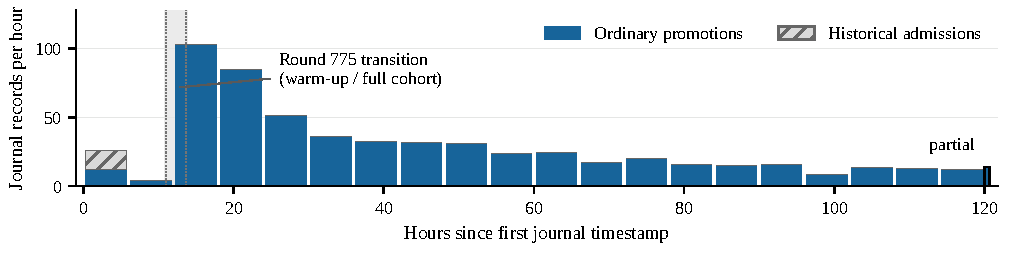
\includegraphics[width=\linewidth,height=1.70in,keepaspectratio]{figures/fig_program_journal_rates.pdf}
  \caption{\textbf{Program-pool journal activity varies across elapsed time.}
  All \num{3490} records through logged round 4406, from 15:06 UTC on
  29 October to the 15:49 UTC capture on 3 November 2026.
  Each bar divides its count by its observed hours: 20 full six-hour bins
  and one partial bin. Blue: \num{3405} ordinary promotions; hatched grey:
  85 historical admissions. The outlined final bin uses its shorter exposure.
  Elapsed time includes work, waits and gaps.
  Ninety early records lack protocol identity; this is not a matched evaluation.
  These rates do not measure proposal success, adapter admission or writer learning.
  Scope: \cref{sec:method-status}.}
  \label{fig:program-journal-rates}
\end{figure*}
